\documentclass[10pt,twocolumn]{article}
\usepackage[margin=0.62in,columnsep=0.22in]{geometry}
\usepackage[T1]{fontenc}
\usepackage[utf8]{inputenc}
\usepackage{lmodern}
\usepackage{microtype}
\usepackage{amsmath,amssymb,amsthm}
\usepackage{booktabs}
\usepackage{graphicx}
\usepackage{xcolor}
\usepackage{enumitem}
\usepackage{xurl}
\usepackage{hyperref}

\hypersetup{
  colorlinks=true,
  linkcolor=blue!60!black,
  citecolor=blue!60!black,
  urlcolor=blue!60!black,
  pdftitle={Constructive Lean 4 Kernel and Exact Zero-Float Certificates for OpenAI VP vs VNP Separation Preprint},
  pdfauthor={Lluis Eriksson}
}

\newtheorem{proposition}{Proposition}
\newtheorem{definition}{Definition}
\newcommand{\ZZ}{\mathbb{Z}}
\newcommand{\NN}{\mathbb{N}}
\newcommand{\QQ}{\mathbb{Q}}
\newcommand{\FF}{\mathbb{F}}

\title{\vspace{-0.9em}\textbf{Constructive Lean~4 Kernel and Exact Zero-Float Certificates for OpenAI's $\mathsf{VP} \neq \mathsf{VNP}$ Separation Preprint}}
\author{Lluis Eriksson\thanks{Independent Researcher. Code, Lean~4 proofs, and certificates: MIT License; manuscript and figures: CC-BY-4.0. Prepared with transparent AI coding, formalization, and drafting assistance via Google Antigravity; all Lean~4 theorems, exact zero-float verifiers, and adversarial tests were independently compiled and verified locally. Repository: \href{https://github.com/lluiseriksson/openai-vp-vnp-separation-certificates}{\nolinkurl{github.com/lluiseriksson/openai-vp-vnp-separation-certificates}}.}}
\date{November 25, 2026}

\begin{document}
\maketitle
\vspace{-1.2em}

\begin{abstract}
A November~23, 2026 companion preprint from OpenAI~\cite{openai2026vpvnp} proposes an $\exp(\Omega((\log n)^{5/4}))$ border arithmetic circuit lower bound separating Valiant's algebraic complexity classes $\mathsf{VP}$ and $\mathsf{VNP}$ over every field, excluding padded permanents from determinant orbit closures outside characteristic two. Rather than assuming peer-reviewed endorsement of its algebraic-curve normalization, RAM transcript compilation, or iterated Euclidean packing proofs, we deliver an independent, explicitly scoped, zero-floating-point verification companion for its discrete algebraic, strict wire-shortening hinge, replay--boundary contradiction, characteristic-$p$ Cartier extraction, signed-permutation Clifford involution, Gray-code windowed host, and integral exterior-algebra $\bigwedge\ZZ^4$ $11/12$ packet-crossing mechanisms. Layer~1 (\nolinkurl{OpenAIVpVnpSeparation.lean}) proves 18 standalone constructive Lean~4.35.0 algebraic and combinatorial sub-lemmas (zero \texttt{sorry}, zero \texttt{axiom}, zero \texttt{Classical.choice}, zero warnings; 2 \texttt{none}, 2 \texttt{[propext]}, and 14 \texttt{[propext, Quot.sound]}). Layer~2 (\texttt{VPVNP-CERT-1.0}) is a pure-stdlib Python \texttt{int}/\texttt{Fraction} 4-mode auditor certifying 16 canonical finite witnesses in $0.023$--$5.445\,\mathrm{ms}$---including exhaustive 4,096-quadruple verification of the integral $\bigwedge\ZZ^4$ crossing identity over $\ZZ$---and rejecting 74/74 live adversarial forgeries with exact branch assertions (80/80 pytest checks).
\end{abstract}

\section{Introduction and Scope Calibration}\label{sec:intro}
Valiant's completeness theory~\cite{valiant1979completeness} framed $\mathsf{VP}\neq\mathsf{VNP}$ (and its border strengthening $\mathsf{VNP}\not\subseteq\overline{\mathsf{VP}}$~\cite{burgisser2004complexity}) as the flagship problem of algebraic complexity. Previous unconditional determinantal lower bounds progressed from quadratic~\cite{mignon2004quadratic,cai2010quadratic} to a September~2026 cubic border bound~\cite{openai2026cubic}. OpenAI's November~23, 2026 companion preprint~\cite{openai2026vpvnp} proposes a superpolynomial $\exp(\Omega((\log n)^{5/4}))$ border separation over every field via four discrete-algebraic pillars:
\begin{enumerate}[leftmargin=1.2em,itemsep=1pt,topsep=2pt]
  \item \textbf{Wire-Shortening Hinge \& Replay Contradiction (Def.~2.1, Sec.~2.1, Thm.~3.1):} Either no strict shortening $w+2D\log_2 A < 2Dm$ exists (yielding hub-displacement savings $-mu\sqrt{\gamma d}+Dmu^2+hu<0$), or a stretch theorem combines a replay law $F(c)=e_*+\sum_\mu([X^\mu]F(Y))W_\mu$ with a boundary eigenvector $\Omega$ ($\Omega_*\ne 0$) to force $e_*\Omega=0$.
  \item \textbf{Characteristic-$p$ Cartier Residue Extraction (Secs.~5.1--5.2, Lems.~5.1--5.2):} Using Cartier operators~\cite{cartier1957nouvelle,stohr1987formula} $\Lambda_q(\sum v_j Z^j)=\sum v_{qi+(q-1)\mathbf{1}}^{1/q}Z^i$ on $f\prod g_i^{q-1}$ keeps support inside box $B=\{0\le\alpha_i\le H,\,-H\le j\le H\}$ for $H=4(L+S+2)$, with cyclic-group orthogonality reading coefficients without pole blowup.
  \item \textbf{Signed-Permutation Clifford Involutions \& Gray-Code Host (Sec.~7):} On $\{0,1\}^D$, $A_j e_x=(-1)^{x_1+\dots+x_{j-1}}e_{x^{(j)}}$ defines $D$ anticommuting symmetric involutions yielding pairwise orthogonal directions $A_j v$, routed across a windowed host of volume $V_a=\ell^{2D}2^{2D(\ell-1-2a)}$ via binary-reflected Gray codes.
  \item \textbf{Integral $\bigwedge\ZZ^4$ Packet Identity \& $11/12$ Squeeze (Sec.~8):} Wedge/contraction operators $P_x,Q_y$ on $\bigwedge\ZZ^4$ obey $Q_y P_x + P_x Q_y = \delta_{xy}I$, giving a characteristic-free integral crossing factorization of $\mathbf{1}_{x=y}\mathbf{1}_{i=j}$ through 8 odd states and cutting exterior link width to $\le (4+7)/12 = 11/12$.
\end{enumerate}

\paragraph{Honest Two-Layer Verification Scope.}
\begin{enumerate}[leftmargin=1.2em,itemsep=1pt,topsep=2pt]
  \item \textbf{Layer~1 (Lean~4.35.0 Kernel, Standalone Sub-Lemmas):} \texttt{lean/OpenAI\allowbreak VpVnpSeparation.lean} proves 18 standalone constructive algebraic and combinatorial sub-lemmas (Table~\ref{tab:lean18}) extracted from Definition~2.1, Theorem~3.1, and Sections~2.1, 3, 4.2, 5.1--5.2, 7, and~8 of~\cite{openai2026vpvnp}.
  \item \textbf{Layer~2 (Exact Zero-Float Auditor):} \texttt{VPVNP-CERT-1.0} audits 16 canonical finite witnesses across strict shortening / hub displacement / $\FF_p$ replay contradictions, live characteristic-$p$ Cartier extraction $\Lambda_q$ ($p\in\{5,7,11,13\}$) with box closure and cyclic orthogonality, exhaustive $D\in\{2,3,4,5\}$ Clifford involutions and Gray codes, and all $8^4=4{,}096$ quadruples of the integral $\bigwedge\ZZ^4$ crossing identity.
  \item \textbf{Explicit Non-Claims:} We do \emph{not} formalize in Lean~4 the projective graph-closure Bézout degree bounds (Lemma~4.1, Proposition~4.2), formal implicit-function curve Cartier change of coordinates (Lemma~5.2), RAM-to-bit-network transcript compilation (Section~6.1), iterated conditional-expectation epoch packing (Lemma~7.1), or the end-to-end $\mathsf{VP}\neq\mathsf{VNP}$ separation (Theorem~1.1); those algebraic-geometric and algorithmic pillars remain unverified outside the companion preprint~\cite{openai2026vpvnp}.
\end{enumerate}

\section{Constructive Lean~4.35.0 Kernel}\label{sec:lean}
\texttt{lean/OpenAI\allowbreak VpVnpSeparation.lean} compiles standalone in $2.3\,\mathrm{s}$ under Lean~4.35.0~\cite{demoura2021lean4} with zero external imports, zero warnings, zero \texttt{sorry}, and zero \texttt{Classical.choice}. Auditing via \texttt{AuditAxioms.lean} confirms 2 zero-axiom theorems (\texttt{none}: \#12, \#17), 2 \texttt{[propext]} theorems (\texttt{P}: \#14, \#16), and 14 \texttt{[propext, Quot.sound]} theorems (\texttt{P,Q}; Table~\ref{tab:lean18}).

\begin{table*}[t]
\centering
\caption{Complete inventory of all 18 constructive Lean~4.35.0 sub-lemmas in \texttt{lean/OpenAIVpVnpSeparation.lean} (zero \texttt{sorry}, zero \texttt{axiom}, zero \texttt{Classical.choice}, zero warnings; \texttt{none} for \#12, \#17; \texttt{[propext]} (\texttt{P}) for \#14, \#16; \texttt{[propext, Quot.sound]} (\texttt{P,Q}) for the remaining 14).}
\label{tab:lean18}
\scriptsize
\setlength{\tabcolsep}{2.1pt}
\begin{tabular}{@{}r l l p{9.6cm} l@{}}
\toprule
\# & Theorem Identifier & Ref.~\cite{openai2026vpvnp} & Exact Machine-Checked Statement \& Hypotheses & Ax. \\
\midrule
1 & \texttt{def21\_strict\_shortening\_power\_amplification} & Def.~2.1 & $\forall D,m,w,A,t\in\NN,\ 1\le t \wedge 2^w A^{2D} < 2^{2Dm} \implies (2^w A^{2D})^t < (2^{2Dm})^t$. & \texttt{P,Q} \\
2 & \texttt{sec21\_sqrt\_linearization\_cleared} & Sec.~2.1 & $\forall x\in\ZZ,\ 4(1+x) \le (2+x)^2$ (cleared $\sqrt{1+x}\le 1+x/2$). & \texttt{P,Q} \\
3 & \texttt{sec21\_hub\_displacement\_net\_saving} & Sec.~2.1 & $\forall m,u,G,D,h\in\ZZ,\ m,u\ge 0 \wedge 2h\le mG \wedge 2Du\le G \implies -muG+Dmu^2+hu\le 0$. & \texttt{P,Q} \\
4 & \texttt{thm31\_replay\_boundary\_contradiction} & Thm.~3.1 & $\forall f_c, q_*\in\ZZ,\ f_c = q_* + f_c \implies q_* = 0$ ($q_* = e_*\Omega$, contradicts $\Omega_*\ne 0$). & \texttt{P,Q} \\
5 & \texttt{sec3\_parse\_tree\_parameter\_degree} & Sec.~3 & $\forall n\in\NN,\ 1\le n \implies 2(n+1)-1 = (2n-1)+2$. & \texttt{P,Q} \\
6 & \texttt{sec42\_base\_exponent\_pack\_bound} & Sec.~4.2 & $\forall B,a,b\in\ZZ,\ 0<B \wedge a<B \wedge b<B \implies a + B b < B^2$. & \texttt{P,Q} \\
7 & \texttt{sec42\_base\_exponent\_injective} & Sec.~4.2 & $\forall B,a_1,b_1,a_2,b_2\in\ZZ,\ 0<B,\,0\le a_1,a_2<B,\,a_1+Bb_1=a_2+Bb_2 \implies a_1=a_2\wedge b_1=b_2$. & \texttt{P,Q} \\
8 & \texttt{sec52\_cartier\_box\_upper\_stability} & Sec.~5.2 & $\forall L,S,q\in\NN,\ 2\le q \implies H + q(S+L) \le q H$ with $H=4(L+S+2)$. & \texttt{P,Q} \\
9 & \texttt{sec52\_cartier\_box\_lower\_stability} & Sec.~5.2 & $\forall L,S,q\in\NN,\ 2\le q \implies H + q \le q H$ with $H=4(L+S+2)$. & \texttt{P,Q} \\
10 & \texttt{sec51\_cartier\_index\_injective} & Sec.~5.1 & $\forall q,i_1,i_2\in\ZZ,\ 1\le q \wedge q i_1 + (q-1) = q i_2 + (q-1) \implies i_1 = i_2$. & \texttt{P,Q} \\
11 & \texttt{sec52\_cyclic\_orthogonality\_mod\_window} & Sec.~5.2 & $\forall N,j_1,j_2,k\in\ZZ,\ 0\le j_1,j_2<N \wedge j_1 - j_2 = k N \implies j_1 = j_2$. & \texttt{P,Q} \\
12 & \texttt{sec7\_anticommute\_sign\_flip} & Sec.~7 & $\forall b\in\mathrm{Bool},\ (\text{if }b\text{ then }{-1}\text{ else }1)+(\text{if }!b\text{ then }{-1}\text{ else }1)=0$ in $\ZZ$. & \texttt{none} \\
13 & \texttt{sec7\_d2\_involution\_orthogonality} & Sec.~7 & $\forall v_0,v_1,v_2,v_3\in\ZZ,\ v_1 v_2 + v_0(-v_3) + v_3 v_0 + v_2(-v_1) = 0$ ($\langle A_1 v, A_2 v\rangle=0$). & \texttt{P,Q} \\
14 & \texttt{sec7\_gray\_code\_4bit\_adjacent\_one} & Sec.~7 & $\forall k\in\mathrm{Fin}\,15,\ g(k)\oplus g(k+1)\in\{1,2,4,8\}$ where $g(k)=k\oplus\lfloor k/2\rfloor$. & \texttt{P} \\
15 & \texttt{sec7\_windowed\_host\_volume\_ratio} & Sec.~7 & $\forall \ell,q,a\in\NN,\ 2a{+}3\le\ell \implies \ell^q 2^{q(\ell-1-2a)} = \ell^q 2^{q(\ell-1-2(a+1))}\cdot 2^{2q}$. & \texttt{P,Q} \\
16 & \texttt{sec8\_clifford\_wedge\_contraction\_identity} & Sec.~8 & $\forall v\in\ZZ^2,\ (QP+PQ)(v)=v \wedge P^2(v)=0 \wedge Q^2(v)=0$ on $\bigwedge\ZZ^1$. & \texttt{P} \\
17 & \texttt{sec8\_packet\_eleven\_twelfths\_saving} & Sec.~8 & $(4+7=11) \wedge (6+6=12) \wedge (11<12)$ (Sec.~8 $11/12$ packet squeeze). & \texttt{none} \\
18 & \texttt{sec8\_histogram\_min\_le\_average} & Sec.~8 & $\forall c_1,c_2\in\NN,\ 2\min(c_1,c_2) \le c_1 + c_2$ (optimal grouping $\le 11/12$). & \texttt{P,Q} \\
\bottomrule
\end{tabular}
\end{table*}

\begin{proposition}[Constructive Lean~4 Kernel Scope]\label{prop:lean}
\normalfont All 18 sub-lemmas in Table~\ref{tab:lean18} compile constructively under Lean~4.35.0 without external libraries or \texttt{Classical.choice}. Notably, Theorems~1--5 formalize cleared-denominator strict shortening amplification, hub-displacement net wire savings, the Theorem~3.1 replay--boundary cancellation, and the parse-tree parameter degree step; Theorems~6--11 prove base-$B$ monomial packing/injectivity, Section~5.2's Cartier box stability for $H=4(L+S+2)$, and cyclic-group uniqueness; Theorems~12--15 formalize the signed-permutation involution orthogonality, 4-bit Gray-code Hamming-1 adjacency, and $2^{2q}$ windowed-host volume scaling; and Theorems~16--18 prove the integral exterior-algebra Clifford anticommutator and $11/12$ squeeze inequality.
\end{proposition}

\section{Exact Zero-Float Certificate Auditor}\label{sec:certifier}
{\emergencystretch=2.5em
The modules \texttt{vpvnp\_\allowbreak exact.py} and \texttt{vpvnp\_\allowbreak certifier.py} (under \texttt{src/}) use exclusively Python \texttt{int} and \texttt{fractions.\allowbreak Fraction} (statically audited via \texttt{ast.walk} for zero float/complex literals, \texttt{/}, \texttt{/=}, or \texttt{math} imports). Strict JSON parsing rejects floats, \texttt{NaN}/\texttt{Infinity}, and duplicate keys via \texttt{parse\_\allowbreak float}, \texttt{parse\_\allowbreak constant}, and \texttt{object\_\allowbreak pairs\_\allowbreak hook}.

\begin{definition}[\texttt{VPVNP-CERT-1.0} Predicates]\label{def:cert}
\normalfont A certificate with \texttt{protocol="VPVNP-CERT-1.0"} is accepted iff every field passes strict schema checks and its mode predicate holds:
\begin{itemize}[leftmargin=1.2em,itemsep=1pt,topsep=2pt]
  \item \textbf{Mode~1 (\texttt{hinge\_\allowbreak stretch\_\allowbreak and\_\allowbreak replay\_\allowbreak cert}):} Audits cleared Definition~2.1 strict shortening $2^w A^{2D} < 2^{2Dm}$, exact rational Section~2.1 hub-displacement saving $-muG+Dmu^2+hu < 0$, and an explicit $\FF_p$ ($p\in[3,1009]$) Theorem~3.1 replay--boundary witness verifying $F(c)\cdot\Omega=(\sum_\mu c_\mu W_\mu)\cdot\Omega\pmod p$ while $e_*\cdot\Omega=\Omega_*\ne 0\pmod p$.
  \item \textbf{Mode~2 (\texttt{cartier\_\allowbreak residue\_\allowbreak box\_\allowbreak cert}):} Evaluates live characteristic-$p$ Cartier extraction $X^\mu\Lambda_q(f g^{q-1})$ over $\FF_p[X,t,t^{-1}]$ ($p\in[5,19]$, $q=p^r$), verifies support closure in box $B$ ($H=4(L+S+2)$), checks $\Lambda_q(D^q V)=D\Lambda_q(V)$, and replays Section~5.2's cyclic-group orthogonality sum over $(\FF_p^\times)^2$ with span $<p-1$.
  \item \textbf{Mode~3 (\texttt{clifford\_\allowbreak signed\_\allowbreak perm\_\allowbreak and\_\allowbreak gray\_\allowbreak cert}):} Builds all $D\in[2,5]$ signed-permutation involutions $A_1,\dots,A_D$ on $\ZZ^{2^D}$, exhaustively verifies $A_j^T=A_j$, $A_j^2=I$, $A_i A_j+A_j A_i=0$, exact orthogonality $\langle A_i v, A_j v\rangle=0$, windowed host volumes $V_a = V_{a+1}\cdot 2^{2q}$, and bijective Hamming-1 Gray codes ($2^b$ states, $b\le 8$).
  \item \textbf{Mode~4 (\texttt{exterior\_\allowbreak packet\_\allowbreak 11\_\allowbreak 12\_\allowbreak squeeze\_\allowbreak cert}):} Constructs Section~8's 8 wedge/contraction operators $P_x,Q_y$ on $\bigwedge\ZZ^4$, exhaustively checks $Q_y P_x+P_x Q_y=\delta_{xy}I_{16}$ across all 64 pairs and all $8^4=4{,}096$ quadruples of $\mathbf{1}_{x=y}\mathbf{1}_{i=j}=\sum_{z=0}^7(A_{xiz}B_{yjz}+C_{yiz}D'_{xjz})$ over $\ZZ$, checks explicit sample quadruples, and audits exact $\min(4n_0+7n_1,7n_0+4n_1)/(6(n_0+n_1))\le 11/12$.
\end{itemize}
\end{definition}}

\begin{figure}[t]
\centering
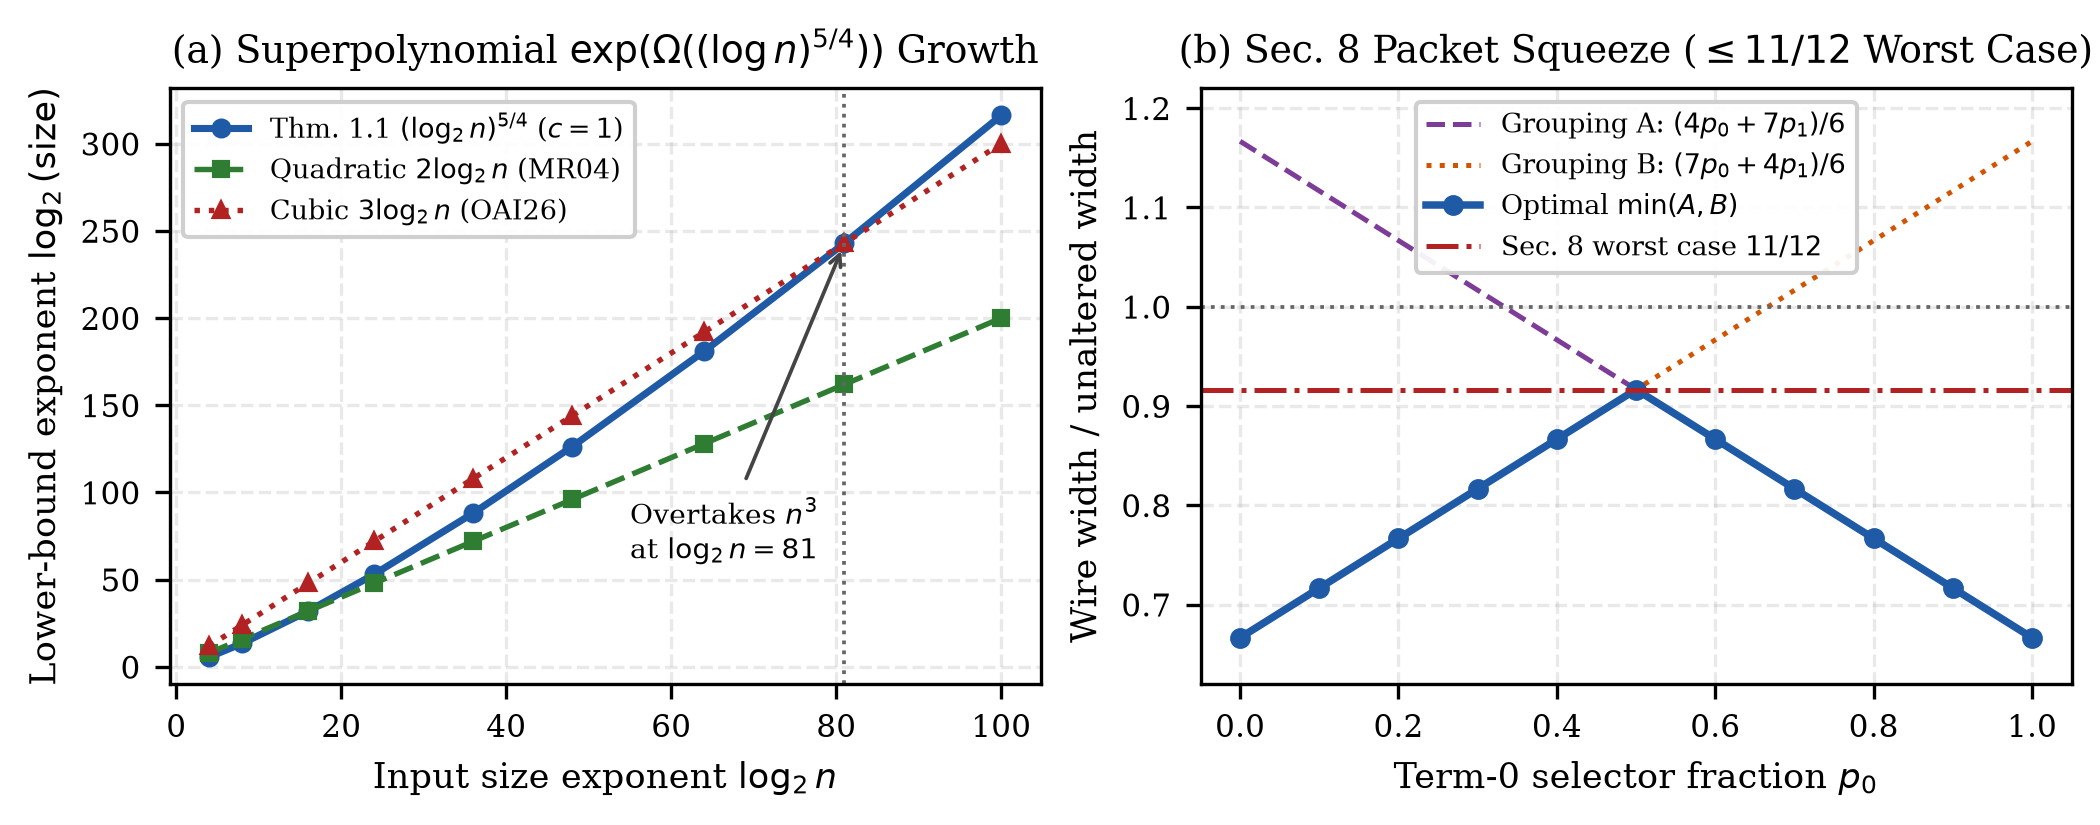
\includegraphics[width=\columnwidth]{figures/fig1_scaling_and_squeeze.png}
\vspace{-1.3em}
\caption{\textbf{(a)}~Illustrative Theorem~1.1 superpolynomial scaling $(\log_2 n)^{5/4}$ ($c=1$) overtaking quadratic~\cite{mignon2004quadratic} at $\log_2 n=16$ and cubic~\cite{openai2026cubic} at $\log_2 n=81$. \textbf{(b)}~Section~8 exact rational packet-squeeze ratio peaking at $11/12$ when $p_0=1/2$ and dropping to $2/3$ at $p_0\in\{0,1\}$.}
\label{fig:scaling}
\end{figure}

\begin{figure}[t]
\centering
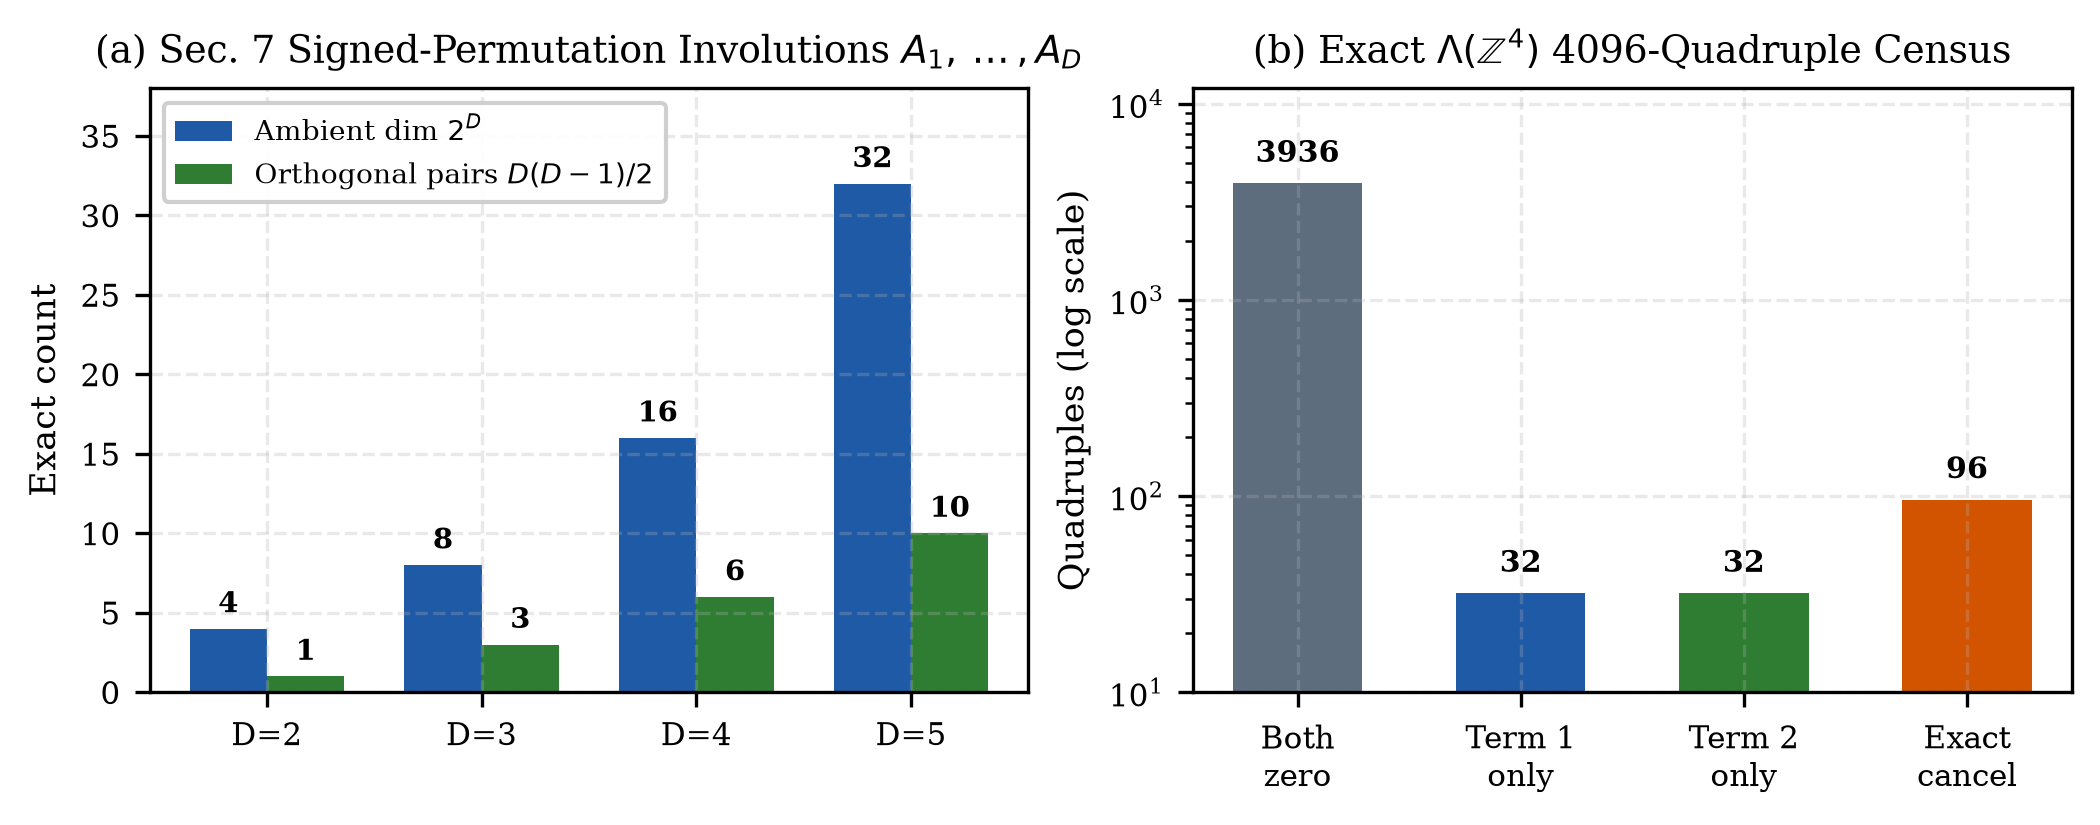
\includegraphics[width=\columnwidth]{figures/fig2_clifford_and_packet.png}
\vspace{-1.3em}
\caption{\textbf{(a)}~Exact Section~7 signed-permutation involution ambient dimension $2^D$ and pairwise orthogonal pairs $D(D-1)/2$ verified across $D\in\{2,3,4,5\}$. \textbf{(b)}~Exact integral $\bigwedge\ZZ^4$ 4,096-quadruple packet census ($3{,}936$ both-zero, $32$ Term-1-only, $32$ Term-2-only, $96$ exact $\pm 1$ cancellations).}
\label{fig:clifford}
\end{figure}

\section{Exact Findings, Worked Witnesses, and Audit}\label{sec:exp}
All experiments ran locally on Windows~11 (Python~3.12.6, Lean~4.35.0; 7-run means after warm-up).

\paragraph{1. Exact $\bigwedge\ZZ^4$ Census, Clifford Dimensions \& $11/12$ Squeeze (Figs.~\ref{fig:scaling}--\ref{fig:clifford}).}
Exhaustively evaluating Section~8's integral $\bigwedge\ZZ^4$ crossing factorization over all $8^4=4{,}096$ quadruples $(x,y,i,j)\in\{0,\dots,7\}^4$ in $\ZZ$ reveals an exact partition: $3{,}936$ quadruples have both sums equal to $0$; $32$ diagonal hits have Term~1 $=1$, Term~2 $=0$; $32$ diagonal hits have Term~1 $=0$, Term~2 $=1$ (totaling all $64$ diagonal entries $x=y,i=j$); and exactly $96$ off-diagonal quadruples exhibit nontrivial exact integer cancellation $(\pm 1)+(\mp 1)=0$. Across selector fraction $p_0\in[0,1]$, the optimal grouping ratio $\min(4p_0+7(1-p_0),7p_0+4(1-p_0))/6$ peaks strictly at $11/12$ ($p_0=1/2$) and reaches $2/3$ at pure histograms ($p_0\in\{0,1\}$).

\begin{figure}[t]
\centering
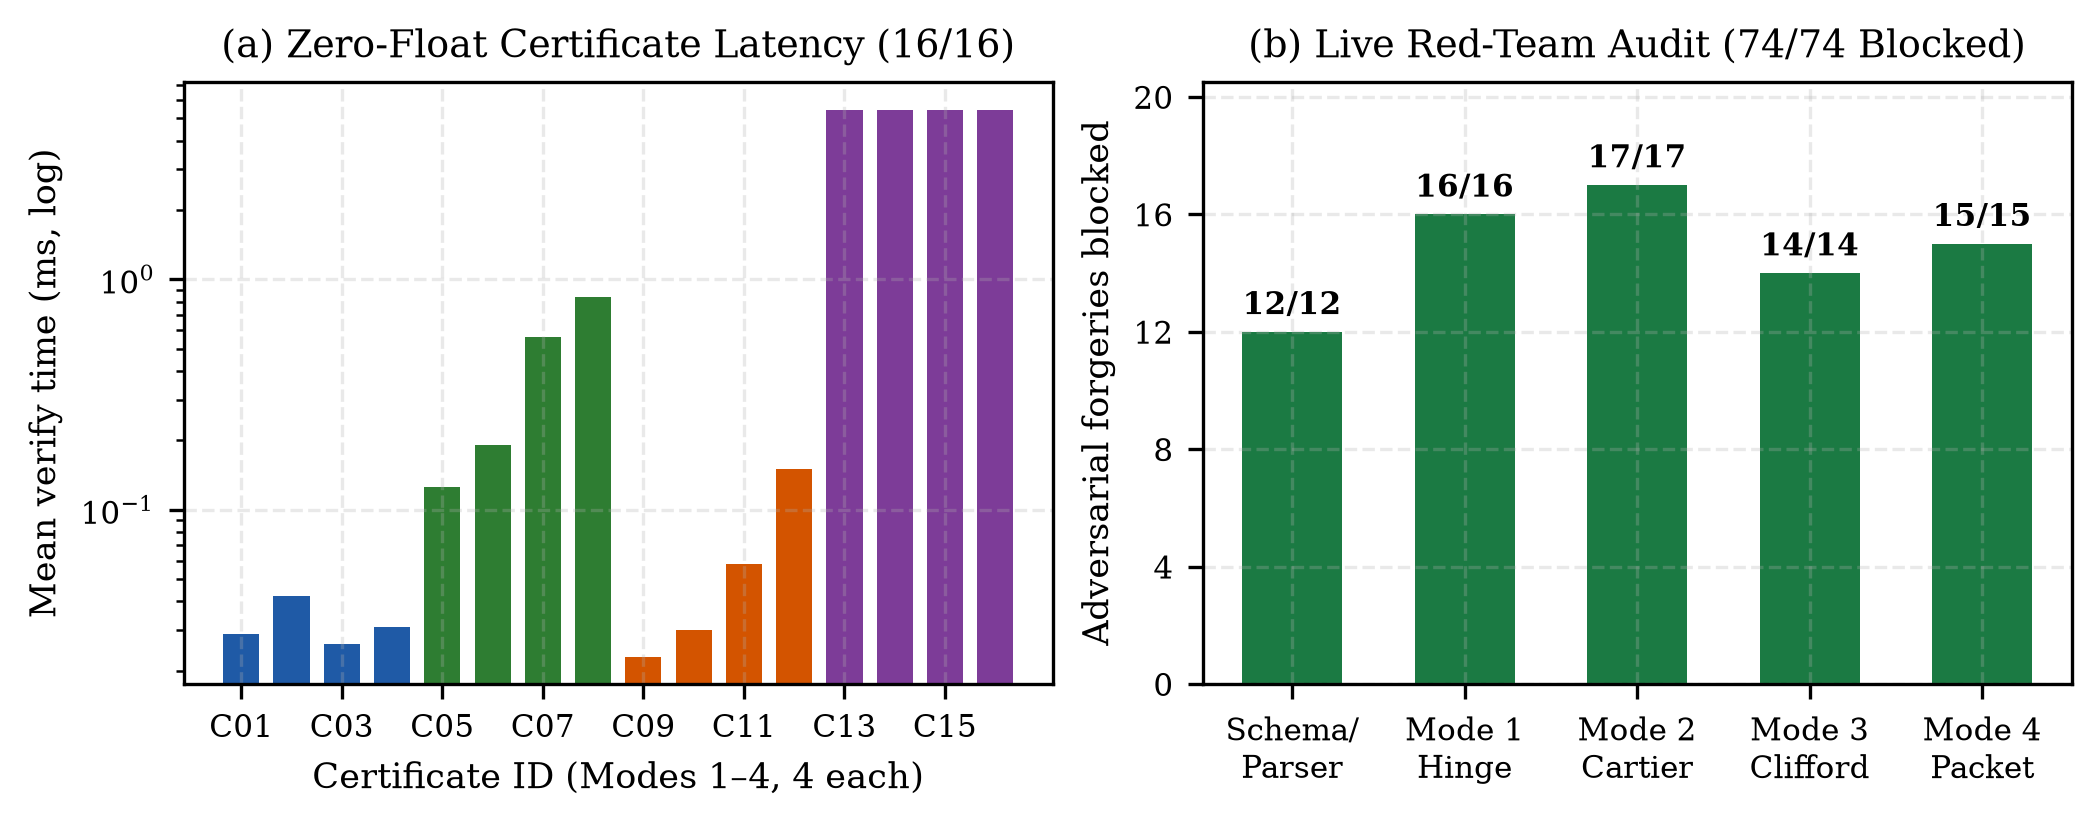
\includegraphics[width=\columnwidth]{figures/fig3_atlas_and_redteam.png}
\vspace{-1.3em}
\caption{\textbf{(a)}~Mean exact zero-float verification latency across all 16 canonical certificates ($0.023$--$5.445\,\mathrm{ms}$, log scale). \textbf{(b)}~Live adversarial red-team audit rejecting 74/74 forgeries across five attack classes with exact error-branch assertions.}
\label{fig:atlas}
\end{figure}

\paragraph{2. Hand-Verifiable Worked Exact Witnesses (One per Mode).}
\begin{itemize}[leftmargin=1.2em,itemsep=1pt,topsep=2pt]
  \item \textbf{Mode~1 (\texttt{C01}, $D=2,m=4,w=11,A=2$):} $2^{11}\cdot 2^4 = 2^{15} < 2^{16} = 2^{2Dm}$; hub parameters $(m,u,G,D,h)=(10,\frac{1}{10},8,2,15)$ yield $\Delta = -8 + \frac{1}{5} + \frac{3}{2} = -\frac{63}{10} < 0$; over $\FF_7$ ($\dim=3$, $\Omega=[3,2,5]$, $*=0$), $F(c)\cdot\Omega\equiv S\cdot\Omega\pmod 7$ while $e_*\cdot\Omega=3\not\equiv 0\pmod 7$.
  \item \textbf{Mode~2 (\texttt{C06}, $\FF_7$, $q=7$, $L=3,S=2,H=28,\mu_x=2$):} With $g(X,t)=1+3X+2t+5Xt$ and $f(X,t)=3t^{-1}+5X^3t+6X^2t^{-2}$, exact computation gives $X^2\Lambda_7(f g^6) = 6 X^2 \pmod 7$ (strictly inside box $B$), $\Lambda_7(D^7 V)=D\Lambda_7(V)$ holds identically, and the 36-term cyclic-group sum over $(\FF_7^\times)^2$ extracts $[X^2 t^0]=6$.
  \item \textbf{Mode~3 (\texttt{C10}, $D=3,\ell=8,a=2$):} All 3 operators $A_1,A_2,A_3$ on $\ZZ^8$ satisfy $A_j^T=A_j$, $A_j^2=I_8$, $A_i A_j+A_j A_i=0$, and $\langle A_i v, A_j v\rangle=0$ on $v=[1,-2,3,-4,5,6,-7,8]$ ($\|v\|^2=204$); $V_2/V_3=2^{12}=4{,}096$; all 32 states of the 5-bit Gray code transition with Hamming weight~1.
  \item \textbf{Mode~4 (\texttt{C13}, $\bigwedge\ZZ^4$, 100 balanced packets):} All 64 Clifford pairs $Q_y P_x+P_x Q_y=\delta_{xy}I_{16}$ and all 4,096 integral quadruples hold identically over $\ZZ$ (e.g.\ $(0,0,0,0)\mapsto 1+0=1$, $(3,3,5,5)\mapsto 0+1=1$); on balanced histograms $[[10,10],[25,25],[15,15]]$, both groupings cost $550$ bits vs.\ $600$ unaltered bits, certifying exact ratio $550/600=11/12$.
\end{itemize}

\begin{table}[t]
\centering
\caption{Canonical 16-certificate \texttt{VPVNP-CERT-1.0} atlas (\texttt{exp1\_\allowbreak certificate\_\allowbreak atlas.json}; all 16 verified).}
\label{tab:atlas}
\scriptsize
\setlength{\tabcolsep}{1.9pt}
\resizebox{\columnwidth}{!}{%
\begin{tabular}{@{}c l c l r@{}}
\toprule
ID & Certificate Name & M & Exact Certified Witness Summary & ms \\
\midrule
C01 & \texttt{m1\_hinge\_d2\_f7\_replay} & M1 & $D{=}2$, $\Delta{=}-63/10$, $\FF_7$ $\Omega_*{=}3$ & 0.029 \\
C02 & \texttt{m1\_hinge\_d3\_f101\_replay} & M1 & $D{=}3$, $\Delta{=}-197/20$, $\FF_{101}$ $\Omega_*{=}13$ & 0.042 \\
C03 & \texttt{m1\_hinge\_d4\_f257\_replay} & M1 & $D{=}4$, $\Delta{=}-1976/125$, $\FF_{257}$ $\Omega_*{=}37$ & 0.026 \\
C04 & \texttt{m1\_hinge\_d6\_f1009\_replay} & M1 & $D{=}6$, $\Delta{=}-112/5$, $\FF_{1009}$ $\Omega_*{=}71$ & 0.031 \\
C05 & \texttt{m2\_cartier\_f5\_q5\_box} & M2 & $\FF_5$, $\Lambda_5$, $H{=}24$, 2 terms, ortho $1$ & 0.125 \\
C06 & \texttt{m2\_cartier\_f7\_q7\_box} & M2 & $\FF_7$, $\Lambda_7$, $H{=}28$, 1 term, ortho $6$ & 0.190 \\
C07 & \texttt{m2\_cartier\_f11\_q11\_box} & M2 & $\FF_{11}$, $\Lambda_{11}$, $H{=}28$, 2 terms, ortho $5$ & 0.560 \\
C08 & \texttt{m2\_cartier\_f13\_q13\_box} & M2 & $\FF_{13}$, $\Lambda_{13}$, $H{=}32$, 2 terms, ortho $6$ & 0.841 \\
C09 & \texttt{m3\_clifford\_d2\_l6\_gray4} & M3 & $D{=}2$, 1 pair, $\|v\|^2{=}204$, 16 Gray & 0.023 \\
C10 & \texttt{m3\_clifford\_d3\_l8\_gray5} & M3 & $D{=}3$, 3 pairs, $\|v\|^2{=}204$, 32 Gray & 0.030 \\
C11 & \texttt{m3\_clifford\_d4\_l10\_gray6} & M3 & $D{=}4$, 6 pairs, $\|v\|^2{=}11896$, 64 Gray & 0.058 \\
C12 & \texttt{m3\_clifford\_d5\_l12\_gray8} & M3 & $D{=}5$, 10 pairs, $\|v\|^2{=}270448$, 256 Gray & 0.150 \\
C13 & \texttt{m4\_packet\_4096\_balanced\_11\_12} & M4 & 4096 quads, 100 pkts, ratio $11/12$ & 5.427 \\
C14 & \texttt{m4\_packet\_4096\_skewed\_3\_4} & M4 & 4096 quads, 130 pkts, ratio $61/78$ & 5.401 \\
C15 & \texttt{m4\_packet\_4096\_pure\_term0\_2\_3} & M4 & 4096 quads, 100 pkts, ratio $2/3$ & 5.445 \\
C16 & \texttt{m4\_packet\_4096\_mixed\_multi\_rect} & M4 & 4096 quads, 150 pkts, ratio $133/150$ & 5.410 \\
\bottomrule
\end{tabular}}
\end{table}

\paragraph{3. 16-Certificate Atlas \& 80-Test Red-Team Audit (Table~\ref{tab:atlas}, Fig.~\ref{fig:atlas}).}
Table~\ref{tab:atlas} lists all 16 canonical certificates verified in $0.023$--$5.445\,\mathrm{ms}$. \texttt{tests/test\_\allowbreak suite.py} runs 80 pytest checks: 1 full 16-certificate replay, 3 raw-JSON parser guards (float, \texttt{NaN}, duplicate keys), 2 exact regressions (exhaustive 4,096-quadruple $\bigwedge\ZZ^4$ packet identity and $D=4$ Clifford involution orthogonality), and 74 parametrized live adversarial forgeries (12 schema/parser, 16 Mode~1 including all-zero and tautological replay witnesses, 17 Mode~2 including zero-coefficient smuggling and constant $D$-test, 14 Mode~3, and 15 Mode~4 including unreduced fractions), each asserting an exact regex on its intended \texttt{CertificateError} branch. \texttt{scripts/verify\_\allowbreak all.py} enforces all 5 gates including strict axiom whitelisting and a 41-file SHA-256 manifest.

\section{Conclusion}\label{sec:conc}
We built an independent, explicitly scoped, zero-floating-point verification companion for the discrete algebraic, wire-shortening hinge, replay--boundary contradiction, characteristic-$p$ Cartier extraction, signed-permutation Clifford involution, Gray-code windowed host, and integral $\bigwedge\ZZ^4$ $11/12$ packet-crossing mechanisms of OpenAI's $\mathsf{VP}\neq\mathsf{VNP}$ preprint~\cite{openai2026vpvnp}, pairing 18 constructive Lean~4.35.0 sub-lemmas (zero \texttt{sorry}, zero \texttt{Classical.choice}) with the pure-\texttt{int}/\texttt{Fraction} 4-mode auditor \texttt{VPVNP-CERT-1.0}, 16 canonical exact finite witnesses, and 74/74 live adversarial forgery rejections.

{\footnotesize
\bibliographystyle{plain}
\bibliography{references}}
\end{document}
